% ============================================================================
% CHAPTER 2 --- PRNet: PAPR REDUCTION VIA DEEP AUTOENCODER
% ============================================================================
\chapter{PRNet: PAPR Reduction via Deep Autoencoder}
\label{ch:prnet}

The limitations of classical SLM identified in Chapter~\ref{ch:ofdm_papr} --- computational complexity, side information overhead, and blind detection difficulty --- motivate a fundamentally different approach.  Rather than searching over a fixed set of phase sequences, Kim et al.~\cite{kim2017novel} proposed the \textbf{PAPR Reduction Network (PRNet)}, the first deep learning-based system for joint PAPR and BER optimisation in OFDM.  PRNet treats the transmitter--channel--receiver chain as a single deep autoencoder: the encoder learns a data-dependent constellation mapping that jointly minimises reconstruction error and PAPR, while the decoder learns the corresponding inverse mapping, eliminating the need for side information.


% ============================================================================
\section{Autoencoder Framework}
\label{sec:autoencoder_framework}
% ============================================================================

\subsection{Communication System as Autoencoder}

In any communication system, the transmitter transforms raw data into a signal suitable for the channel, and the receiver undoes that transformation to recover the original data.  This structure maps directly onto the autoencoder paradigm~\cite{kim2017novel}: the encoder corresponds to the transmitter, the bottleneck corresponds to the physical channel (which adds noise and distortion), and the decoder corresponds to the receiver.

The key insight of PRNet is that if both the transmitter and receiver are designed as jointly trained neural networks with the channel model placed between them, the system can be trained end-to-end to minimise any differentiable objective --- including PAPR~\cite{kim2017novel}.


\subsection{PRNet Architecture Overview}

PRNet inserts two trainable Deep Neural Networks (DNNs) around the standard IFFT/FFT pair~\cite{kim2017novel}.  The \textbf{encoder} (transmitter-side DNN) replaces the standard constellation mapper: instead of mapping bits to fixed QPSK or QAM points, it produces complex subcarrier values specifically shaped to yield low peaks after the IFFT.  The \textbf{decoder} (receiver-side DNN) replaces the standard constellation de-mapper and directly reconstructs the original data from the received noisy frequency-domain subcarriers.

It is important to note that the IFFT and FFT remain fixed, standard mathematical operations within the PRNet pipeline.  The encoder replaces the constellation mapper, not the IFFT itself~\cite{kim2017novel}.

\begin{figure}[H]
    \centering
    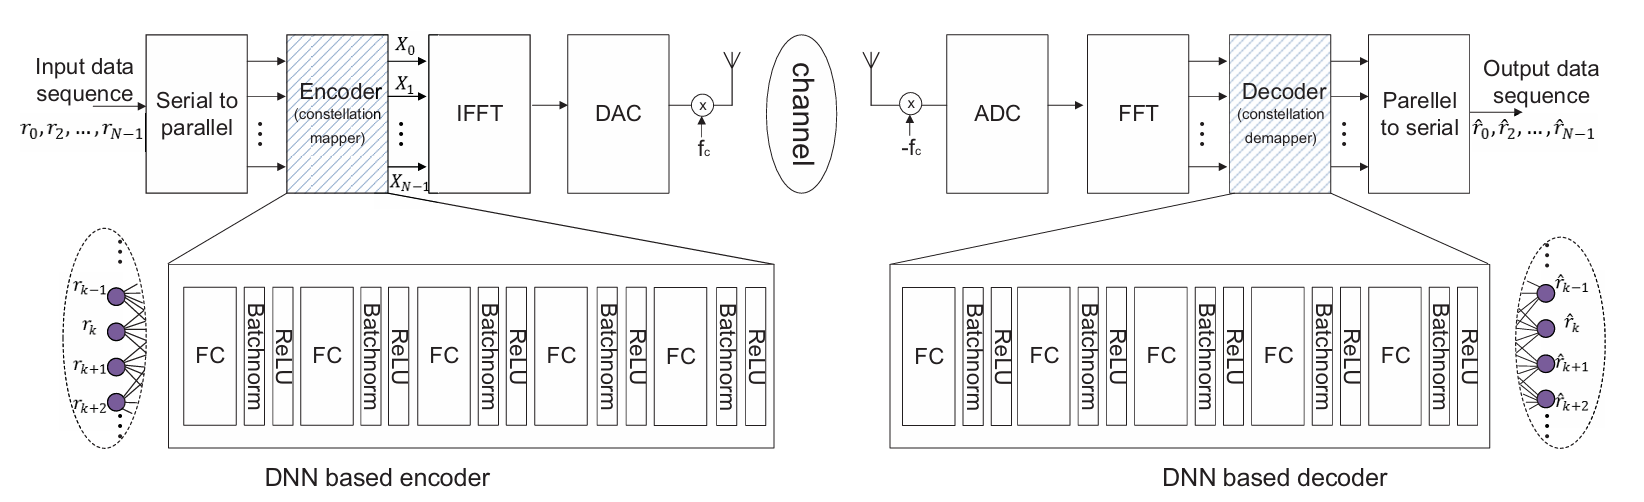
\includegraphics[width=0.95\linewidth]{Figures/PRNet/prnet_architecture.png}
    \caption{Structure of the PRNet system with DNN encoder and DNN decoder. Both consist of fully connected (FC) layers with Batch Normalization and ReLU activation.  The encoder shapes the constellation before the IFFT to reduce PAPR; the decoder reconstructs the transmitted symbols after the channel and FFT. Reproduced from~\cite{kim2017novel}.}
    \label{fig:prnet_architecture}
\end{figure}

Because the encoder and decoder are trained jointly over the full training process, the decoder's weights implicitly encode the complete knowledge of the encoder's mapping.  No explicit side information is transmitted between transmitter and receiver, eliminating both the bandwidth overhead and the catastrophic failure mode associated with SI errors in classical SLM~\cite{kim2017novel}.


\subsection{Joint Subcarrier Processing}

In standard OFDM with QPSK, the constellation mapping is performed independently per subcarrier: each pair of bits maps to one of four fixed points.  PRNet fundamentally changes this by employing a fully connected encoder, where every output subcarrier value is a function of the \emph{entire} input block.  This holistic processing enables the encoder to detect input patterns that would produce high PAPR under standard mapping and to compensate by adjusting all subcarrier amplitudes and phases jointly~\cite{kim2017novel}.


% ============================================================================
\section{System Model}
\label{sec:system_model}
% ============================================================================

The complete PRNet signal chain can be expressed as~\cite{kim2017novel}:
\begin{keyresult}
\begin{equation}
    \hat{\bm{r}}
    = g \circ \mathrm{FFT} \circ \mathbb{H} \circ \mathrm{IFFT}
      \circ f(\bm{r}),
\end{equation}
\end{keyresult}
where $f$ denotes the encoder, $g$ denotes the decoder, $\mathbb{H}$ represents the channel, and $\bm{r}$ and $\hat{\bm{r}}$ are the input and reconstructed output vectors, respectively.  The following subsections describe each stage.


\subsection{Input Representation}

The system considers $N = 64$ subcarriers with QPSK modulation ($M = 4$ constellation points per subcarrier), yielding $N \times \log_2 M = 128$ bits per OFDM symbol~\cite{kim2017novel}.  The symbol index for each subcarrier is $r_k \in \{0, 1, 2, 3\}$, and the full input vector is $\bm{r} = [r_0,\, r_1,\, \dots,\, r_{N-1}]^T$.

In the neural network implementation, each symbol index $r_k$ is represented as a one-hot vector of length $M = 4$, and these vectors are concatenated to form the network input~\cite{kim2017novel}:
\begin{equation*}
    \bm{r}_{\mathrm{input}} \in \mathbb{R}^{NM} = \mathbb{R}^{256}.
\end{equation*}
One-hot encoding ensures that the network treats each symbol index as an independent category without imposing a spurious ordinal relationship~\cite{kim2017novel}.


\subsection{Encoder: Learned Constellation Shaping}

The encoder is a deep neural network that maps the one-hot input vector $\bm{r}_{\mathrm{input}} \in \mathbb{R}^{NM}$ to a vector of $2N = 128$ real numbers representing the real and imaginary parts of $N$ complex subcarrier values~\cite{kim2017novel}:
\begin{equation*}
    f(\bm{r};\,\theta_f) \in \mathbb{R}^{2N},
\end{equation*}
where $\theta_f$ denotes all learnable weights and biases.  The \textbf{unstacking operator} $\mathcal{C}(\cdot) : \mathbb{R}^{2N} \to \mathbb{C}^{N}$ converts these to complex symbols:
\begin{equation*}
    \bm{X}_{\mathrm{enc}} = \mathcal{C}\bigl(f(\bm{r};\,\theta_f)\bigr)
    \in \mathbb{C}^{N},
\end{equation*}
where the $k$-th encoded symbol is $X_{\mathrm{enc},k} = f(\bm{r})_{2k} + j \cdot f(\bm{r})_{2k+1}$. These symbols are not constrained to any standard constellation grid; they are continuous-valued complex numbers shaped by the encoder to produce low-PAPR waveforms after the IFFT~\cite{kim2017novel}.


\subsection{OFDM Modulation}

The encoded symbols are modulated onto the subcarriers via the standard IFFT~\cite{kim2017novel}:
\begin{keyresult}
\begin{equation}
    x[n] = \sum_{k=0}^{N-1} X_{\mathrm{enc},k}\, e^{\,j2\pi nk/N},
    \qquad 0 \le n \le N-1.
\end{equation}
\end{keyresult}
This is the standard IFFT operation; the only difference from conventional OFDM is that the input symbols $X_{\mathrm{enc},k}$ are the encoder's learned values rather than fixed constellation points.

For accurate continuous-time PAPR estimation, the frequency-domain vector can be zero-padded from length $N$ to $NL$ before computing an $NL$-point IFFT, where $L$ is the oversampling factor.  With $N = 64$ and $L = 4$, this produces 256 time-domain samples~\cite{kim2017novel}.


\subsection{Channel Model}

After OFDM modulation, the time-domain signal passes through the wireless channel, modelled as~\cite{kim2017novel}:
\begin{equation*}
    \bm{y} = \mathbb{H}(\bm{x}) + \bm{\epsilon},
\end{equation*}
where $\mathbb{H}$ denotes the channel effects (Rayleigh fading~\cite{kim2017novel}) and $\bm{\epsilon}$ is additive white Gaussian noise (AWGN).

From the neural network's perspective, the channel is a fixed mathematical function within the computation graph.  During training, the channel is simulated by generating random noise and fading coefficients.  Since these operations (addition, multiplication) are differentiable, gradients from the loss function propagate backward through the channel during backpropagation~\cite{kim2017novel}.


\subsection{Decoder}

At the receiver, the FFT recovers the frequency-domain subcarriers:
\begin{equation*}
    \bm{Y} = \mathrm{FFT}(\bm{y}) \in \mathbb{C}^{N}.
\end{equation*}
The decoder DNN processes these received symbols via the \textbf{stacking operator} $\mathcal{S}(\cdot) : \mathbb{C}^{N} \to \mathbb{R}^{2N}$, which interleaves real and imaginary parts, and produces the reconstructed output~\cite{kim2017novel}:
\begin{equation*}
    \hat{\bm{r}} = g\bigl(\mathcal{S}(\bm{Y});\,\theta_g\bigr)
    \in \mathbb{R}^{NM},
\end{equation*}
where $\theta_g$ denotes the decoder's learnable parameters.  The output consists of scores for each possible symbol index; the final decision is made by selecting the index with the largest score for each subcarrier.


\subsection{Signal Dimension Summary}

\begin{table}[H]
    \centering
    \caption{Summary of PRNet signal dimensions for the one-hot formulation~\cite{kim2017novel}.}
    \label{tab:prnet_shapes}
    \begin{tabular}{@{} l l l @{}}
        \toprule
        \textbf{Symbol} & \textbf{Domain / Shape} & \textbf{Meaning} \\
        \midrule
        $\bm{r}$              & $\mathbb{R}^{NM}$ ($256$)
            & One-hot encoded input \\
        $f(\bm{r})$           & $\mathbb{R}^{2N}$ ($128$)
            & Encoder output (stacked I/Q) \\
        $\bm{X}_{\mathrm{enc}}$ & $\mathbb{C}^{N}$ ($64$)
            & Encoded complex subcarrier symbols \\
        $x[n]$                & $\mathbb{C}^{NL}$ ($64L$)
            & IFFT output (time-domain waveform) \\
        $\bm{y}$              & $\mathbb{C}^{NL}$ ($64L$)
            & Received signal (after channel) \\
        $\bm{Y}$              & $\mathbb{C}^{N}$ ($64$)
            & FFT output (received subcarriers) \\
        $\hat{\bm{r}}$        & $\mathbb{R}^{NM}$ ($256$)
            & Decoder output (reconstructed scores) \\
        \bottomrule
    \end{tabular}
\end{table}


% ============================================================================
\section{Network Architecture}
\label{sec:network_architecture}
% ============================================================================

Both the encoder and decoder are constructed from repeated sub-blocks, each consisting of a Fully Connected (FC) layer, Batch Normalization (BN), and ReLU activation, applied in sequence~\cite{kim2017novel}.

\subsection{Sub-Block Structure}

Each sub-block transforms an input vector $\bm{h}^{(\ell-1)}$ into an output vector $\bm{h}^{(\ell)}$ through three operations:

\textbf{Fully Connected Layer.} A linear transformation $\bm{y}_{\mathrm{FC}} = \bm{W}_m \bm{h}^{(\ell-1)} + \bm{b}_m$, where $\bm{W}_m \in \mathbb{R}^{d_{\mathrm{out}} \times d_{\mathrm{in}}}$ and $\bm{b}_m \in \mathbb{R}^{d_{\mathrm{out}}}$. The hidden layers use $d_{\mathrm{out}} = 2048$ nodes~\cite{kim2017novel}.

\textbf{Batch Normalization.} Normalises the FC output to zero mean and unit variance within each training mini-batch, then applies learnable scale ($\gamma$) and shift ($\beta$) parameters~\cite{kim2017novel}:
\begin{equation*}
    |\bm{y}_{\mathrm{FC}}|_{\mathrm{norm}}
    = \gamma \cdot
    \frac{\bm{y}_{\mathrm{FC}} - \mathbb{E}[\bm{y}_{\mathrm{FC}}]}
         {\sqrt{\mathrm{Var}[\bm{y}_{\mathrm{FC}}] + \nu}}
    + \beta,
\end{equation*}
where $\nu = 0.001$ prevents division by zero.  BatchNorm stabilises training and allows the use of higher learning rates.

\textbf{ReLU Activation.} The Rectified Linear Unit $\phi(x) = \max(x, 0)$ provides the nonlinearity essential for the network to learn the complex, non-convex constellation shaping required for PAPR reduction~\cite{kim2017novel}.

The complete sub-block transformation is:
\begin{equation*}
    \bm{h}^{(\ell)}
    = \phi\!\Bigl(
        \mathrm{BN}\bigl(\bm{W}^{(\ell)}\bm{h}^{(\ell-1)}
        + \bm{b}^{(\ell)}\bigr)
    \Bigr),
    \qquad \phi(\cdot) = \mathrm{ReLU}(\cdot).
\end{equation*}


\subsection{Encoder and Decoder Topology}

The encoder consists of $L_f = 5$ FC--BN--ReLU sub-blocks~\cite{kim2017novel}:
\begin{keyresult}
\begin{equation}
    f(\bm{r})
    = \phi_{L_f}\!\Bigl(
        \bigl|\bm{W}_{L_f}^f\,
        \phi_{L_f-1}\bigl(\cdots
            \phi_1\bigl(|\bm{W}_1^f\,\bm{r}
                        + \bm{b}_1^f|_{\mathrm{norm}}\bigr)
        \cdots\bigr)
        + \bm{b}_{L_f}^f\bigr|_{\mathrm{norm}}
    \Bigr).
\end{equation}
\end{keyresult}

The decoder has the same topology ($L_g = 5$ sub-blocks) with its own independent set of weights.  The final output layer of each network is a plain FC layer with linear activation (no ReLU), as the outputs must be unconstrained real values~\cite{kim2017novel}.


% ============================================================================
\section{Training Methodology}
\label{sec:training}
% ============================================================================

\subsection{Loss Function}

PRNet optimises two competing objectives simultaneously: reconstruction accuracy (low BER) and peak suppression (low PAPR).  The reconstruction loss measures the Mean Squared Error (MSE) between the original and reconstructed vectors~\cite{kim2017novel}:
\begin{keyresult}
\begin{equation}
    \mathcal{L}_1(\bm{r},\hat{\bm{r}})
    = \frac{1}{NM}\|\bm{r} - \hat{\bm{r}}\|_2^2
    = \frac{1}{NM}\sum_{i=0}^{NM-1}\bigl(r_i - \hat{r}_i\bigr)^2.
\end{equation}
\end{keyresult}

The PAPR penalty directly measures the peak-to-average power ratio of the time-domain waveform~\cite{kim2017novel}:
\begin{keyresult}
\begin{equation}
    \mathcal{L}_2(\bm{r})
    = \mathrm{PAPR}\{x[n]\}
    = \frac{\displaystyle\max_{0 \le n \le NL-1} |x[n]|^2}
           {\displaystyle\frac{1}{NL}\sum_{n=0}^{NL-1}|x[n]|^2}.
\end{equation}
\end{keyresult}

The joint loss function is a weighted combination~\cite{kim2017novel}:
\begin{keyresult}
\begin{equation}
    \mathcal{L}(\bm{r},\hat{\bm{r}})
    = \mathcal{L}_1(\bm{r},\hat{\bm{r}}) + \lambda\,\mathcal{L}_2(\bm{r}),
\end{equation}
\end{keyresult}
where $\lambda > 0$ controls the trade-off between reconstruction accuracy and PAPR reduction.  Larger $\lambda$ values produce stronger PAPR reduction at the expense of higher BER.  The paper adopts $\lambda = 0.01$~\cite{kim2017novel}.

\begin{keyinsight}[The BER--PAPR Trade-off]
    The parameter $\lambda$ governs a fundamental trade-off: more aggressive PAPR reduction requires greater constellation distortion, which degrades the decoder's ability to distinguish between symbol classes.  This trade-off is not a limitation specific to PRNet but a physical constraint of the OFDM system.
\end{keyinsight}


\subsection{Two-Stage Training Procedure}

PRNet employs denoising autoencoder training, where noise at corruption level $\eta$ (noise-to-signal ratio) is injected during training to force the decoder to learn robust decision boundaries~\cite{kim2017novel}:
\begin{equation*}
    \eta = \frac{\mathbb{E}\bigl[|\epsilon|^2\bigr]}
                {\mathbb{E}\bigl[|\bm{r}|^2\bigr]}.
\end{equation*}

Selecting $\eta$ involves a trade-off: too little noise yields overly tight decision boundaries that fail under real channel conditions, while too much noise prevents the decoder from learning to distinguish adjacent constellation points.  Kim et al.\ employ a two-stage procedure~\cite{kim2017novel}:

\begin{enumerate}
    \item \textbf{Stage~1 --- Corruption level selection:} Train multiple models using only the reconstruction loss $\mathcal{L}_1$ ($\lambda = 0$) for a range of $\eta$ values. Evaluate BER across a full SNR sweep and select the $\eta$ yielding the lowest overall BER.  The paper identifies $\eta^\star = -15$~dB~\cite{kim2017novel}.

    \item \textbf{Stage~2 --- Joint training:} Fix $\eta = \eta^\star = -15$~dB and train the final model with the full joint loss $\mathcal{L} = \mathcal{L}_1 + \lambda\,\mathcal{L}_2$.
\end{enumerate}

Stage~1 establishes robust reconstruction capability before Stage~2 introduces the PAPR objective, preventing the encoder from distorting the constellation before the decoder has developed adequate noise-handling foundations.

\begin{algorithm}[H]
    \DontPrintSemicolon
    \SetAlgoLined
    \SetKwInOut{Input}{Input}
    \SetKwInOut{Output}{Output}
    \Input{Candidate corruption levels $\{\eta\}$, PAPR weight $\lambda$,
           steps $T$, batch size $B$}
    \Output{Trained parameters $(\theta_f,\theta_g)$}
    \BlankLine
    \tcp{Stage 1: select $\eta^\star$ using $\lambda=0$}
    \ForEach{$\eta$ in $\{\eta\}$}{
        Initialise PRNet parameters $(\theta_f,\theta_g)$\;
        \For{$t=1$ \KwTo $T$}{
            Sample a batch of $B$ random QPSK symbol indices $\to \bm{r}$\;
            Forward pass: $\hat{\bm{r}} \leftarrow
                \mathrm{PRNet}(\bm{r};\theta_f,\theta_g,\eta)$\;
            Compute $\mathcal{L}_1(\bm{r},\hat{\bm{r}})$ and update
                $(\theta_f,\theta_g)$ via Adam\;
        }
        Evaluate BER over an SNR sweep and record result for this $\eta$\;
    }
    Select $\eta^\star$ that minimises BER\;

    \BlankLine
    \tcp{Stage 2: joint training at $\eta^\star$}
    Initialise the final PRNet parameters $(\theta_f,\theta_g)$\;
    \For{$t=1$ \KwTo $T$}{
        Sample a batch of $B$ random QPSK symbol indices $\to \bm{r}$\;
        Forward pass: obtain $\hat{\bm{r}}$ and time-domain $x[n]$\;
        Compute $\mathcal{L} = \mathcal{L}_1(\bm{r},\hat{\bm{r}})
            + \lambda\,\mathcal{L}_2(x[n])$\;
        Update $(\theta_f,\theta_g)$ via Adam on $\nabla\mathcal{L}$\;
    }
    \caption{Two-stage PRNet training procedure~\cite{kim2017novel}.}
    \label{alg:prnet_training}
\end{algorithm}


\subsection{End-to-End Differentiability}

Training requires gradients to flow from the loss function through the decoder, FFT, channel, IFFT, and encoder.  For the AWGN channel ($\bm{y} = \bm{x} + \bm{\epsilon}$), the noise term does not depend on the encoder's parameters, so $\partial\mathcal{L}/\partial\bm{x} = \partial\mathcal{L}/\partial\bm{y}$.  For multiplicative fading channels ($\bm{y} = h\bm{x} + \bm{\epsilon}$), the gradient is scaled by the fading coefficient.  The IFFT and FFT are linear operations whose gradients are their respective transposes.  The $\max$ function in the PAPR loss is differentiable almost everywhere, with gradient equal to 1 at the position of the maximum and 0 elsewhere.  Consequently, gradients propagate cleanly through the entire system~\cite{kim2017novel}.


% ============================================================================
\section{Inference and Deployment}
\label{sec:inference}
% ============================================================================

\subsection{Inference Procedure}

After training, the encoder and decoder weights are frozen.  Inference consists of a single forward pass through the encoder, a standard IFFT for OFDM modulation, transmission over the physical channel, FFT demodulation, and a single forward pass through the decoder.  The encoder is a deterministic function: the same input always produces the same output, with no search, candidate comparison, or trial-and-error involved~\cite{kim2017novel}.


\subsection{Generalisation}

The encoder is not a lookup table but an algebraic function (composition of matrix multiplications and ReLU operations) whose parameters were optimised to perform well in general.  During training, the network processes $500{,}000 \times 400 = 200$ million random OFDM symbols, a vanishingly small fraction of the $2^{128} \approx 3.4 \times 10^{38}$ possible input sequences.  The network nevertheless handles all possible inputs through generalisation: it learns the underlying geometric principles of PAPR avoidance rather than memorising specific input--output pairs~\cite{kim2017novel}.

The fully connected architecture produces dense mixing, where each encoded subcarrier depends on the entire input block.  This enables the decoder to exploit a non-standard, globally shaped constellation geometry.  However, this property should not be interpreted as a formal frequency-diversity scheme; the system's robustness to channel effects is limited to the distribution encountered during training~\cite{kim2017novel}.


% ============================================================================
\section{Simulation Results}
\label{sec:simulation_results}
% ============================================================================

\subsection{Simulation Setup}

\begin{table}[H]
    \centering
    \caption{PRNet simulation parameters~\cite{kim2017novel}.}
    \label{tab:prnet_params}
    \begin{tabularx}{\linewidth}{@{} l X @{}}
        \toprule
        \textbf{Parameter} & \textbf{Value} \\
        \midrule
        Number of subcarriers ($N$)        & 64 \\
        Modulation                         & 4-QAM/QPSK \\
        Network input representation       & $NM=256$ one-hot entries \\
        Hidden processing blocks per DNN   & 5 \\
        Hidden nodes per layer             & 2048 \\
        Activation function                & ReLU (hidden), Linear (output) \\
        Batch normalisation                & Yes, after every FC layer \\
        Optimiser                          & Adam \\
        Learning rate                      & $10^{-4}$ \\
        Batch size                         & 400 \\
        Training steps                     & 500{,}000 \\
        Optimal corruption level ($\eta^\star$) & $-15$~dB \\
        PAPR weight ($\lambda$)            & 0.01 \\
        CCDF evaluation size               & 50{,}000 random OFDM sequences \\
        PTS comparison                     & 4 sub-blocks, 4 phase factors \\
        \bottomrule
    \end{tabularx}
\end{table}


\subsection{BER Performance}

\begin{figure}[H]
    \centering
    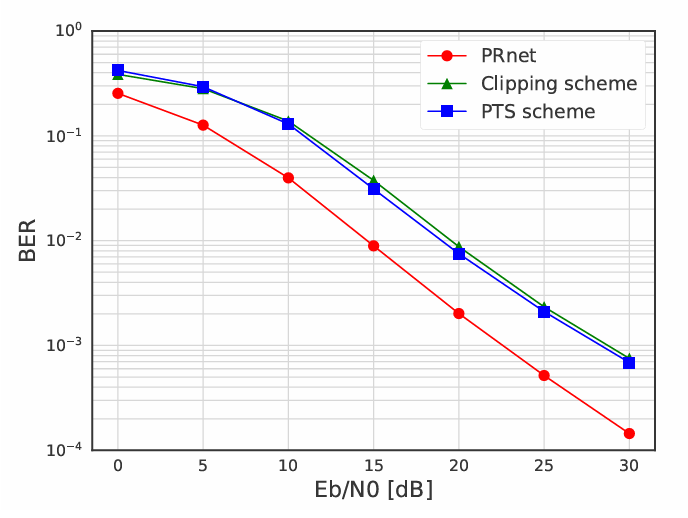
\includegraphics[width=0.55\linewidth]{Figures/PRNet/prnet_ber.png}
    \caption{BER vs.\ SNR of conventional PAPR reduction schemes and PRNet. PRNet achieves the lowest BER among the plotted schemes because the jointly trained encoder--decoder pair effectively learns a form of implicit joint source-channel coding.  Reproduced from~\cite{kim2017novel}.}
    \label{fig:prnet_ber}
\end{figure}

The BER results show that clipping introduces in-band distortion which becomes the dominant error source at high SNR.  PTS is distortionless in principle but requires side information and multiple IFFT computations. PRNet achieves BER lower than the plotted baselines because the encoder shapes the constellation in a way that the jointly trained decoder can exploit, effectively learning an implicit coding gain under the simulated channel~\cite{kim2017novel}.


\subsection{PAPR Reduction}

\begin{figure}[H]
    \centering
    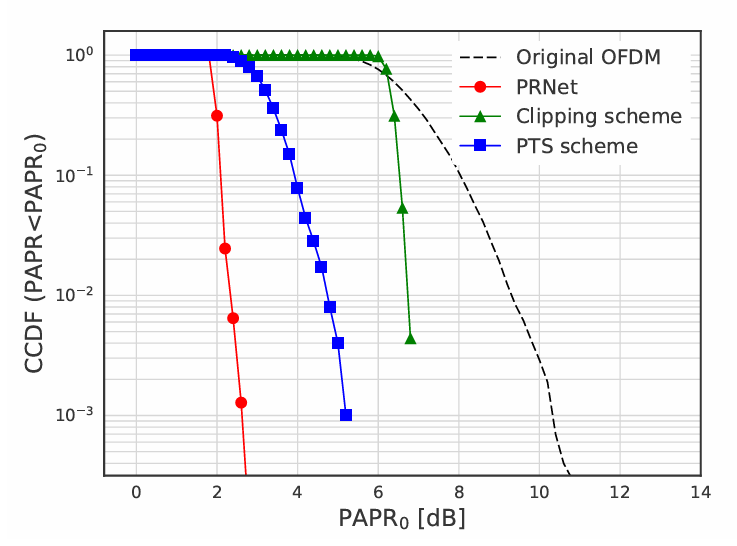
\includegraphics[width=0.55\linewidth]{Figures/PRNet/prnet_ccdf.png}
    \caption{CCDF of PAPR as reported by the original PRNet paper. The PRNet curve is significantly shifted to the left compared to conventional OFDM.  Reproduced from~\cite{kim2017novel}.}
    \label{fig:prnet_ccdf}
\end{figure}

The CCDF plot demonstrates that PRNet substantially reduces PAPR.  The paper reports that the probability of PAPR exceeding 3~dB is less than 0.1\%~\cite{kim2017novel}, allowing the HPA to operate with substantially less input back-off.

It should be noted that the released implementation computes the CCDF using a peak-amplitude proxy ($10\log_{10}\max_n |x[n]|$) rather than the standard power-PAPR definition.  Standard power-PAPR evaluation yields a PRNet value near 6~dB at $\mathrm{CCDF} = 10^{-3}$, which is still a significant reduction from the conventional OFDM baseline of 10--11~dB, but less extreme than the paper's visual figure suggests.


\subsection{Effect of Corruption Level}

\begin{figure}[H]
    \centering
    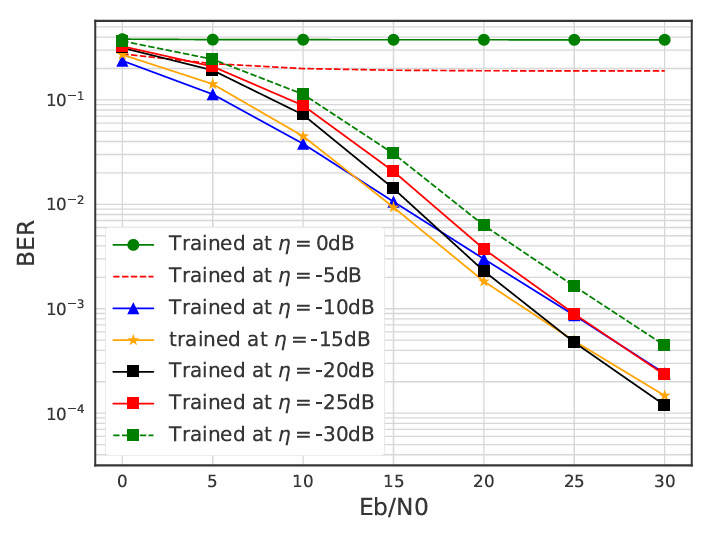
\includegraphics[width=0.55\linewidth]{Figures/PRNet/prnet_ber_corruption.png}
    \caption{BER of PRNet trained at different corruption levels $\eta$. The model trained at $\eta = -15$~dB consistently yields the lowest BER across the entire SNR range. Reproduced from~\cite{kim2017novel}.}
    \label{fig:prnet_ber_corruption}
\end{figure}

The results validate the two-stage training procedure: models trained at very low corruption levels ($\eta = -30$~dB) develop overly tight decision boundaries and fail under real channel noise, while models trained at excessive corruption ($\eta = 0$~dB) cannot learn meaningful boundaries. The optimal corruption level $\eta^\star = -15$~dB yields the lowest BER across all tested SNR values~\cite{kim2017novel}.


\subsection{BER--PAPR Trade-off}

\begin{figure}[H]
    \centering
    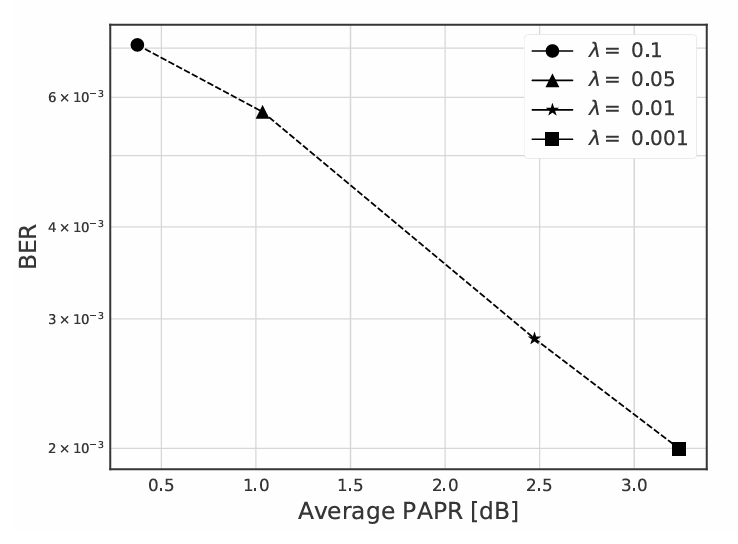
\includegraphics[width=0.55\linewidth]{Figures/PRNet/prnet_ber_papr_lambda.png}
    \caption{BER vs.\ average PAPR by varying $\lambda$ at SNR $= 20$~dB. Larger $\lambda$ reduces PAPR but increases BER, confirming the fundamental trade-off. Reproduced from~\cite{kim2017novel}.}
    \label{fig:prnet_ber_lambda}
\end{figure}

As $\lambda$ increases, PAPR decreases monotonically while BER increases, confirming the fundamental tension between these objectives.  At $\lambda = 0.01$, the paper reports a practical operating point with meaningful PAPR reduction and competitive BER~\cite{kim2017novel}.


\subsection{Computational Complexity}

At inference time, PRNet replaces the $U$-fold search of SLM/PTS with a single forward pass.  The per-pass complexity is $\mathcal{O}(L \cdot K \cdot M)$, where $L$ is the number of layers, $K = 2048$ is the hidden dimension, and $M$ is the input dimension.  This cost is fixed and does not grow with the number of candidates $U$~\cite{kim2017novel}.

\begin{table}[H]
    \centering
    \caption{Execution time comparison for different PAPR reduction methods~\cite{kim2017novel}.}
    \label{tab:prnet_timing}
    \begin{tabular}{@{} l r @{}}
        \toprule
        \textbf{Method} & \textbf{Execution time ($\mu$s)} \\
        \midrule
        PTS                         & 2{,}890 \\
        Clipping and filtering      & 1{,}415 \\
        PRNet (without parallelism) & 2{,}304 \\
        PRNet (with GPU)            & 480 \\
        \bottomrule
    \end{tabular}
\end{table}

With GPU acceleration, PRNet is approximately 6 times faster than PTS and 3 times faster than clipping and filtering, while achieving better BER and PAPR performance~\cite{kim2017novel}.


% ============================================================================
\section{Limitations}
\label{sec:limitations}
% ============================================================================

Despite its contributions, PRNet presents several limitations that define the research agenda for subsequent work.

\textbf{Scalability.} The fully connected architecture scales poorly with the number of subcarriers. The first encoder FC layer has $d_{\mathrm{in}} \times 2048$ weights, where $d_{\mathrm{in}} = NM$ in the one-hot formulation.  For $N = 64$ and $M = 4$, this yields 524{,}288 parameters in the first layer alone.  Scaling to practical large-FFT systems would require alternative architectures such as convolutional, unfolding, or attention-based designs~\cite{kim2017novel}.

\textbf{Channel mismatch.} Performance is tightly coupled to the channel model used during training. Extending PRNet to frequency-selective channels, imperfect channel state information, and rapidly time-varying scenarios remains an open problem~\cite{kim2017novel}.

\textbf{Configuration dependence.} Any change in modulation order ($M$), number of subcarriers ($N$), or pilot structure changes the network's input/output dimensions or signal statistics, requiring architectural modifications or complete retraining.

\textbf{PAPR metric ambiguity.} The released code computes the PRNet CCDF using a peak-amplitude proxy rather than the standard power-PAPR definition, producing results that appear more favourable than standard evaluation.

\textbf{Interpretability.} The learned constellation shaping is encoded in millions of weight values. Understanding the specific structure the network has discovered, or providing worst-case guarantees, is extremely difficult compared to transparent methods like SLM.


% ============================================================================
\section{Related Work}
\label{sec:related_work}
% ============================================================================

PRNet established the autoencoder paradigm for PAPR reduction.  Subsequent works build on this foundation while addressing specific limitations: constrained autoencoders that learn SLM-style phase factors rather than unconstrained nonlinear mappings, signal-cancellation frameworks that achieve PAPR reduction without requiring a jointly trained decoder, and adaptations of the autoencoder architecture to optical OFDM systems with fibre-channel effects~\cite{kim2017novel}.


% ============================================================================
\section{Summary}
\label{sec:ch2_summary}
% ============================================================================

This chapter presented PRNet, the first deep learning-based system for joint PAPR and BER optimisation in OFDM.  The autoencoder architecture replaces the constellation mapper and de-mapper with jointly trained DNNs, eliminating the multi-IFFT search and side information overhead of classical SLM.  The two-stage training procedure identifies the optimal corruption level before introducing the PAPR penalty, and the resulting system achieves both lower BER and lower PAPR than the classical baselines at competitive computational cost.  The limitations identified --- scalability, channel sensitivity, configuration dependence, and interpretability --- define the direction for future work in this area.
